\chapter{双枪少女}

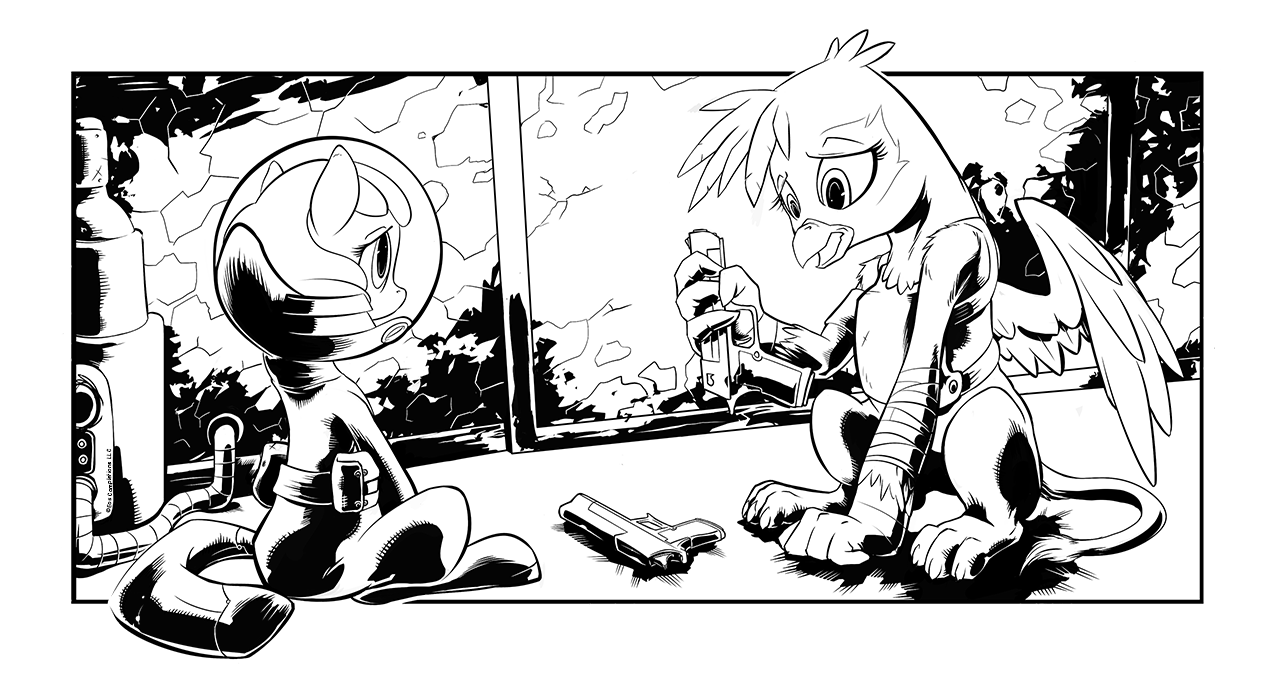
\includegraphics[width=\linewidth]{image06.png}


\begin{intro}
    兰斯洛特,加拉哈德还有我一直等到日落,然后突然杀出去,把那些法兰西鬼子打得措手不及——他们甚至没来得及拿起武器!\footnote{这里是亚瑟王故事的节选}
\end{intro}

{\rt 晚上好,我最亲爱的听众们!你正在收听的是孤狼的52电台!这个频道有你们最想知道的52国道大新闻!}

然后是一阵班卓琴的短暂音乐声。

{\rt 让我们先从正事开始讲起,你们想要知道太阳是什么样子吗?问白苹果们吧!昨晚一个巨大的光球就在盐块城东边十公里左右的距离炸响了!很幸运的是,那里基本都是辐射蜥蜴和遗弃的窝棚。不过那光线就算在隧道镇甚至赤兔领土也能看得一清二楚。如果你觉得这件事非常疯狂,我要和你说,这个可是昨晚百老汇歌舞秀的一部分!首先我们看到一个载满尸鬼的气球升空——就是在盐块城圆顶肆虐的那些尸鬼!陪伴他们升空的是一个叫快乐帕比的小马表演的灯光秀,还真是个奇怪的名字,是吧,不过这个名字似乎听起来很耳熟吧?没错,她就是嘉年华的那位小幼驹!}

然后是一阵胜利的号角声。

{\rt 那么大家问我了,这新闻有什么意义?给那些『懒得听故事直接听结果的观众』一个简单版本!以后在盐块城郊外再也不会受到野生动物和尸鬼的袭击啦!}

然后喇叭里面传来一个拉枪栓的声音和一发枪响,然后还有一个非常硬汉的声音说:「{\rt 后会有期,丫头。}」

{\rt 我爱死这个小家伙了,两个城镇的问题被一个不会脱防辐射服的小幼驹解决了!就算我不是未卜先知,我也知道她一定会往南前进,那么……接下来是什么呢?她要重新开放隧道么?我说,孩子,如果你碰巧路过盐泥沼泽的荒芜之地,你一定要来看你的头号粉丝!我很想知道头盔里面的小脸有多么可爱!好了,现在和往常一样,来点超酷的音乐吧!}

\begin{song}
左一个小马,右一个小马

Here's a pony there's a pony

\medskip

还有一个小小小马,

and another little pony

\medskip

可爱的小马,快乐的小马,

funny pony party pony

\medskip

这就是小小小马!

pony pony sprite\dots
\end{song}

\horizonline

\daytimeplace{5}{16:45 PM}{165战指,盐泥沼泽}{165Th Brigade field Headquarter, Salt Marshes}

% TODO: 检查翻译

「关了那鬼音乐,老娘都听不到那死鬼是不是在外面了!」年轻的狮鹫怒气冲天地瞪了帕比一眼。

「但是……很好听啊!你真是个坏脾气小鸡!」小雌驹皱着眉头又抱她的萍琪派玩偶去了,「别担心丝尾,她没发火,只是累了。」

狮鹫赫瑞塔走到帕比身边,拎着她的头盔把她抓起来,好让她看着自己的双眼。「老娘最后一次警告你!是狮鹫!不是小鸡!外面老大一只蝎尾狮想把我们当晚餐,你丫还一个劲儿地找茬儿,是不是想死啊你?」少女的尖叫声又慢慢低了下去,「我真希望我老爸赶紧回来,」她叹了口气,「或许他能帮我逃出去,然后我就再也不用看你那张傻兮兮的脸了。」

「人家才不傻……你才是个坏心眼猫,我再也不想做你的朋友了!」

「{\mt 警告,检测到敌对狮鹫,距离3米,威胁等级:高。}」

「唉,别说啦,声音先生……」帕比做出一副夸张的厌恶表情转过身去。

「你让谁别说了?你和谁讲话呢?」狮鹫忽然睁大了眼睛。「你那东西还带无线电?」狮鹫跳到帕比背上用力想脱掉她的头盔。「我们可以呼叫支援啊!快叫我爸爸,他在 \SI{90.08}{Hz}!呼号炙红!」

幼驹被吓了一跳,「喂喂,等等!我要先问问声音先生!他住在这个防护服里面,操作那些奇怪的东西。」小雌驹举起蹄子嘘走赫瑞塔,不过狮鹫已经躲一边去了。

「等等,什么声音先生?这防护服能说话?」

「当然可以!这是最好的太空服!而且它超级聪明!」帕比自豪地笑着。

「对哦……」赫瑞塔嗤之以鼻,「比你聪明多了。」

「当然,比我聪……」小雌驹的笑容变成怒容。「喂喂!怎么能这么说人家!」

狮鹫被她逗乐了,「你丫这么简单的招都会中么,你这小鬼太搞笑了,自己承认自己比个香蕉睡衣都蠢!」赫瑞塔说着用爪子弹了一下小雌驹。

「喂喂喂!干什么呢!坏心眼小鸡!如果不是你爹地伤得那么重,我早就教训你了哦!」

赫瑞塔一下愣住了,盯着帕比问:「我老爸怎么了?你怎么认识我老爸?」

帕比看着少女充满希望和惊恐的表情,觉得自己应该非常非常非常谨慎地选择自己下一句话。

「呃……上次我见他的时候,他状态是……死亡,或许他现在已经好点儿了?」幼驹满怀稚气和天真地微笑着。

「我……老爸……死了?你怎么知道的?你什么时候看见他的?这不……这不可能!他是最棒的!不可能死的!你绝对看错了!快跟我说这不是真的!」狮鹫拔出她的白色手枪,带着黄色条纹的枪口指着幼驹的鼻尖。「快说!你看错了!」

赫瑞塔发红的眼睛死盯着帕比粉红的眸子——幼驹虽然有点结巴,但是那双闪闪发光的粉色双眸绝对不可能撒谎,她只是一个稚气未脱的小孩子。

「我……我不知道,他……只是跟我说……他想和你说,他非常非常非常想和你在一起,他很抱歉,所以我超级快地跑过来找你,因为我觉得他看起来伤得很重,而且我很想我妈妈……」

「住口!」赫瑞塔一爪子把帕比拍飞到了墙上,跪在地上把头深深埋在双臂之间,不敢面对残酷的现实。「这不是……这不是真的……我爸爸……是最厉害的赏金猎人……他绝对没事的,他一定会赶来救我……我……我……」

一个金属碰撞的铿锵声让少女抬起了头。

帕比站在赫瑞塔面前,幼驹什么也没说,只是把那柄带着红色条纹的黑色手枪放在狮鹫面前,然后又蜷缩回房间的角落。

「黑玫瑰……」年轻的飞行员吃惊地瞪大眼睛看着面前的枪。「不……不……不会……不可能的……这不是……」她又一次看着穿黄衣的小马。「拜托……求你告诉我……这不是真的!我只是在做噩梦!」

帕比皱着眉头低下了头,「我……我不知道……如果这是一个噩梦的话,那我醒来的时候,妈咪一定会在我身边安慰着我,所以……我希望这也只是一个长长的噩梦……」幼驹又叹了口气,「但是,我不觉得这是……」

「肏!」赫瑞塔用爪子抓起那个手枪,和她自己的点45手枪完全一模一样,除了颜色。「到底发生了什么?为什么你会在现场?」\emph{冷静点儿,赫瑞塔,别情绪化了,你应该问清楚她情况,你可以做得更好,你必须做得更好!}

% NOTE: . -> 点

「我看到天上好像有四个小鸡……」

「不!准!叫!老!娘!小!鸡!我们是狮鹫!比你们这些蠢小马厉害几百倍!你要再叫老娘一次小鸡,那就是你丫这辈子的最后一句话了!懂不懂?」狮鹫拎着帕比的脖子,另一只爪子举着枪顶着她大吼道。

幼驹的眼睛充满了恐惧,她挣扎了两下想要逃跑,但是很快就放弃了,她大哭起来。「我……我很抱歉狮鹫小姐!我会乖乖的!别……别欺负我……」

赫瑞塔点点头把她放下来,「这下好多了,有四个狮鹫在天上飞,然后呢?」刚才的怒气似乎冲散了狮鹫的其它情绪,让她可以更认真地听帕比讲下去。

快乐帕比结结巴巴地继续她的故事,不想让可怕的狮鹫再发火。「就是刚刚,我和朋友正顺着路走,然后天上……呃……天上……开始好像是他们在跳舞一样但是他们看起来好多受伤掉了下来我走过去看他们最后掉下来的一个跟我说给你那个黑东西然后和你说他很抱歉他想往南去我戳戳他想让他醒来但是他还是一直睡我真的真的真的很努力去戳他让他醒来但是他就是不醒来!请别对我发火我真的真的真的想让他好起来但是声音先生和我说他已经『死亡了』而且……而且……」幼驹后退了几步,缩成一团,用前蹄抱着头盔。「请不要欺负我,我真的没有恶意,我只想帮忙!对不起!」

\emph{肏,算了,她只是个孩子!}狮鹫摇了摇头,自己的怒火也开始消退,这个幼驹估计都不知道『小鸡』对狮鹫而言是侮辱性的称呼……趁她还没给自己惹上真正的麻烦之前,某狮鹫还是好好教她吧。

「那个某狮鹫还能是谁?」赫瑞塔长叹一口气,轻轻拍着帕比的头盔,「好了没事了,真的,叫我赫瑞塔,或者赫瑞好么?你只是有点……没教养,别担心,我教你就是。现在我们还是想个办法出去吧。」

「但是……你刚刚还对我发火……」帕比还是双蹄抱头的蹲防姿势。

「我没生气,真的……做个好孩子,站起来,好不好?」

「但是我叫你小鸡还说你是坏蛋……」幼驹小心地露出脸。

「别那么叫了行不行?我也对你吼过了,我们扯平了,可以吧?」

「所以……所以我们还能做朋友?」帕比满怀希望地问。

狮鹫叹了口气,「对,我们还是朋友……现在让我安静一会儿,我好想个办法出来。」

对,办法,说起来简单做起来……好吧,不是一般的难,但是至少这些话还是让帕比再次变回了快乐模式。幼驹点了点头坐在楼梯上,狮鹫看着外面,那猎食者估计在哪里躲着,等她们自己走到空旷地去。

「没戏……要是我有比枪更厉害点的东西,或许还能拼一下,不过如果……」狮鹫回头看着帕比,「我说,你不会刚好带着爆炸物或者重武器吧?」

「我有一个石头!超耐磨!」帕比自豪地把「命运之石」展示给赫瑞塔看。

狮鹫不屑地嗤之以鼻,「还真是CNM!抱歉,我可不想把我的命赌在这块蠢石头上。」

雌驹歪着她的头,一脸不解地看着她最喜欢的武器。「小石石,我才不觉得你蠢……不过现在你还是回包包里睡觉吧。」

「拜托!老娘正在想个正儿八经的主意呢!别在这儿和你包包里面的东西挨个吻别了,你他喵的能做点有用的么……比如……比如说……算了,你还是去和你的闪尾玩去吧。」

「丝尾!」

「对,就是那玩意……一边玩去……」

「好的好滴好的!茶点五分钟就来!」帕比坐在楼梯上开始和她的萍琪派娃娃聊天。

「无论如何……」狮鹫开始低声自言自语,「附近没有任何掩体,我估计只能带着那东西跑个几分钟,好吧,我们真的需要重火力……」赫瑞塔无奈的叹着气,「简直太扯了,外面的坦克装满各种炮弹,我们蹲在这里,只有三把点45手枪和一个……石头……」

% NOTE: . -> 点

这个时候,帕比正在把她的玩偶放在一枚大号坦克炮弹弹头上,然后用另一个当做茶壶来沏茶。「喏,你杯子里面要6块还是8块方糖?呃……你有杯子么?」

「不,谢了,我不要,我想我有个办法了。」狮鹫完全懒得去看幼驹在做什么,她一边继续观察着外面一边说:「我先跑出去吸引那蝎尾狮的注意,等他开始追我的时候,你冲到最近的坦克里面,你最好快点,因为我不能带他跑太久,你要找的是高爆弹头,那东西又大又亮,像一个尖头大水壶,而且上面有个红条,懂了么?」

「呃……好吧……」帕比看了看她蹄子上的『水壶』然后耸了耸肩把那东西放一边,「那你能帮我看好丝尾么?」

「我觉得我们出去之后你的玩偶也不会跑哪儿去的,你丫就给老娘利索点儿,去坦克里面拿个有红头的大『茶壶』回来,等你搞定这事儿之后我们再继续下一步计划。」狮鹫蹲下来,活动一下筋骨准备冲出去,她现在需要自己是最佳状态。

「但是……她会害怕!」幼驹继续冒着傻气。

「帕比,闪尾只是个玩偶!她不可能害怕!」赫瑞塔扭头抓起那个萍琪派玩偶,在幼驹面前晃着说:「看到没?她在笑!她没关系的!回来时候说不定她还能给我们办个……高爆弹?」狮鹫瞪大眼睛看着帕比玩具的那个椅子。「呃……你从哪儿找到这个的?」

黄衣幼驹开心地说:「炫彩大厅!软气给我的!」

「不是……我是说这个椅子……」

「哦,这个啊……在那个坏掉的大铁马车里面,闪闪发光哦,我拿了好几个。」看着狮鹫的表情,帕比于是又说:「你想要吗?」

赫瑞塔眼角抽搐着,「这……真好……第一步完成了……现在我们开始第二步……」

「但是我们什么都……」

「好了,啥都别说……我们,第二步,懂了吗?」狮鹫觉得自己的自控能力越来越好了。「你仔细听好,我把那个大坏蛋引到这个塔的门口,当那蝎尾狮探头进来的时候,你就把这个弹头丢进他嘴里,然后我就打爆他,然后乒,炸飞他的头,然后坏蛋就死翘翘了!」

帕比皱了皱眉头,「就是说……我把茶壶丢进他嘴里然后电影就结束了?」

「电影啥?哦对,把那东西丢进蝎尾狮嘴里,然后我处理剩下的事,好了,你准备好,别吓坏了,懂?」

「好的好的……」幼驹抱起弹头然后躲在墙后面,赫瑞塔谨慎地展开翅膀探出头。

不过一分钟,外面就传来枪声,还有一大堆帕比完全没有听过的精彩狮鹫方言骂街,幼驹超超超好奇外面到底发生了什么,但是赫瑞塔叫她乖乖呆好。现在幼驹觉得有点麻烦了——如果赫瑞塔发现她溜出去了那么一定会很生气,她生气起来可害怕了……但是帕比觉得外面一定有什么超级酷的事情发生,而且生怕错过了。

「或许稍微稍微稍微看一下下……」听着外面的怒吼声和枪声,幼驹抱着她的高爆弹,小心地爬到了门口。「就看一下下……一下下……绝对没关系的。」

「哎,啥都看不见!这不公平……」

忽然一个残影飞快地冲过门口跑到房间的对面大叫着。「就是现在!」

「现在啥?」帕比有点奇怪地问。

嗷呜!!!

随着一阵水泥碎块飞溅,蝎尾狮脑袋冲进门来,但是身体却卡在门框上进不来,帕比发现自己就距离那巨兽的尖牙只有几厘米的距离,让她吓得尖叫一声坐了一个屁股蹲。

「你丫搞什么呢!快丢那劳什子然后趴下!」赫瑞塔惊恐的大叫起来,「给老娘动起来!」

黄色幼驹大叫一声发射了炮弹——那弹头画了一个小小的抛物线,而帕比则以一个更大的抛物线向后蹦了出去,在弹头落在野兽面前的时候,狮鹫举起了枪。

乒!乒!乒!

% NOTE: 呯 -> 乒

三发射击,三发命中,三发跳弹。

「肏!谁尼玛把弹壳做这么厚枪都打不穿!」

双枪少女一边骂着一边把手枪里面的所有子弹都倾泻在那个破弹头上,但是却什么都没发生。

「肏,肏,肏,没用!」赫瑞塔收起双枪然后拿出第三把手枪,那把黑色并且有着红色条纹的手枪——这把枪和她的另外两把没什么区别,她把一梭子子弹打在蝎尾狮鼻子上,终于让那个怪物退缩了一下。

「我想他正在把入口弄大。」帕比又后退了几步,而且看起来没那么害怕了,幼驹轻轻敲着自己头盔下巴的位置,看起来好像在分析战局。「他好厉害哦!」

野兽血红的双眼瞪着赫瑞塔,显然他不打算再回外面蹲伏去了——即使这意味着他要把整个指挥塔拆掉来抓狮鹫,而且他也正在拆了,虽然拆得有点慢。

「在那傻站着干啥,赶紧滚过来!」狮鹫一边给手枪装子弹一边吼着。「就算老娘手枪打不响,但是如果打中引信还是能把你的屁股炸开花,你丫给我找个掩体蹲好!」

「吟新……是啥?」

赫瑞塔忽略帕比的又一个傻问题,从掩体跳出来,双枪瞄准那个炮弹的引信,「说拜拜吧,你这个……」

就在这时,年轻的飞行家注意到蝎尾狮正在低着头弓着身子做出飞扑准备动作,等赫瑞塔飞到空中的时候才知道蝎尾狮的弹跳能力有多好,但是已经太迟了——她连骂街的机会都没有,一瞬间就被蝎尾狮的爪子像拍苍蝇一般从天上拍了下来。

赫瑞塔被蝎尾狮有力的爪子按住了肩膀,她无助地挣扎着,被蝎尾狮撕扯着。

快乐帕比也同样惊恐地尖叫起来,幼驹想后退,但是自己的臀部已经碰到了墙壁,蝎尾狮非常非常可怕,它正在伤害赫瑞!

那一瞬间,帕比看到的不是蝎尾狮,而是一张双眼闪着光的粉红色金属面具。

「\emph{求你……哈哈哈……别让我……哈哈哈……笑了……\footnote{嘉年华的瑞吉}}」

帕比双眸之中点燃了粉色的火焰,她举起蹄子大喊:「石头!」

「命运之石」立刻飞到她的蹄子上,幼驹高高跃起冲向那个野兽。

「放开她!快放开她!」

蝎尾狮被黄色的小小奇袭打乱了节奏,他把自己的旧猎物丢到了一边,怒吼着转向小小幼驹。然后张开血盆大口,随着清脆的咔嚓一声,黄色的小雌驹消失在怪物嘴中。

赫瑞塔尽力保持自己的清醒,挣扎着爬上楼梯,而那头蝎尾狮得意地吼叫声为帕比的命运盖棺定论。

「不……不,已经太迟了……快逃命吧……别回头看……」重伤的狮鹫一边自言自语,一边爬上楼梯,只是走这几步身上的伤口就让她痛得快昏过去了,身后蝎尾狮正在疯狂地怒吼着,估计正在撕扯那可怜小家伙的尸体,赫瑞塔拿出一瓶治疗药水一饮而尽,然后转头看着楼梯下面。但是她只能看到一片粉红色的烟雾,接下来伤口的剧痛和失血让她失去了意识。

……

现在,还是让我们为那个非常不走运的蝎尾狮默哀一分钟吧。

这就是为什么说『绝对不要随便乱吃东西』,因为那肉显然已经变质了。

\horizonline

\daytimeplace{6}{00:45 AM}{165战指,盐泥沼泽}{165Th Brigade field Headquarter, Salt Marshes}

「{\mt 系统重启完毕,所有功能恢复,自检系统上线,目标001:快乐帕比,雌性陆马,目标已死亡,体征状况稳定,完毕!}」

懒洋洋地睁开眼睛,帕比打了个哈欠。「外面还黑洞洞的呢……」睡觉的时候还被什么重物压着,这让她很不开心。

「发生什么事情了?小鸡呢?大坏猫呢?」

「{\mt 分析中,监测到敌对生物,距离6米,赫瑞塔,威胁等级:可忽略。}」

一个红点在罗盘上闪烁着。

「傻声音,赫瑞不是敌对圣姑!」

那个红点变成了粉色。

「很好,我们出……咦?」蹬着蹄子却发现自己没在移动,帕比这才注意到她挂在灰白色的杆子上。花了吃奶的力气,帕比好不容易从蝎尾狮的骨头堆里面钻了出来,那个野兽的骨架看起来已经和墙壁的颜色一样,似乎已经和墙壁融为一体,而那个长满利齿的白色骷髅头仿佛正在绝望地嚎叫,翅膀的骨头也伸开,似乎它不顾一切想要逃开那吞噬它的致命粉云。

帕比走到了赫瑞塔身边,但是狮鹫却一动不动地躺在地上。

「声音先生……她是不是……你知道的那个……死了?」

「{\mt 分析中,否定,目标失去意识。}」

「哦……这表示她会好起来?」

「{\mt 肯定,目标恢复中。}」

「好滴!」这句话对于帕比来说就够了,她开心地隔着头盔和赫瑞塔吻别。

「我很抱歉,但是我必须走了,小鸡,我妈妈还在粉箭头的末端呢!」

帕比走了几步,但是又退了回来。她觉得只是吻别似乎不够,幼驹拿出萍琪派玩偶然后放在狮鹫的爪子中。

「听好,丝尾,帮我照顾赫瑞塔,别让坏事发生在她身上。」

这次没什么问题了,帕比开心地跑到外面,然后捡起自己的滑板车。

「嘿,能来点音乐吗?」

\begin{song}
在丛林中,密密的丛林中。

In the jungle, the mighty jungle,

\medskip

今晚狮子在沉睡。

the lion sleeps tonight!

\medskip

在丛林中,恬静的丛林中。

In the jungle, the quiet jungle,

\medskip

今晚狮子在沉睡。

the lion sleeps tonight\dots
\end{song}

\horizonline

\daytimeplace{6}{10:00 AM}{狮鹫陨落之地,盐泥沼泽}{Griffon's Fall, Salt Marshes}

不用铲子挖坑本身就是一种折磨,而在泥泞之中,用你自己的爪子挖自己父亲的墓穴,简直就是……

大颗的泪水顺着狮鹫的喙滑落,每一次她想要挖出泥土,就会有更多的泥水落回来。但是她却无言地继续挖着,他从来没让她哭过,他是最厉害的最顶尖的佣兵,但是现在他死了,被鹰爪佣兵\footnote{鹰爪佣兵 (Talons):狮鹫公国被英克雷吞并之后,流亡的狮鹫组成的大型佣兵组织,大多数狮鹫都属于鹰爪佣兵}杀害了。

赫瑞塔把他拖进浅浅的墓穴里面,尸体在泥泞之中发出湿软的声音,女儿看着自己父亲的鲜血渐渐渗入泥土之中,努力把自己的泪水咽下去。

他喵的……这个墓穴甚至不能装下他。

「这不公平,把我自己孤零零地丢在这里……我现在还能去哪儿?」赫瑞塔叹息着,她想要发火,但是却一点怒气都没有。他已经走了……还能怎样。

「为什么……」

肏!

肏蛋!

狮鹫慢慢地用泥土和附近的碎石将墓穴盖好。她拿出黑色的手枪,迟疑了一下又放了回去,然后拔下自己的三根羽毛,然后放在她父亲永远安眠的胸口附近。

「跟老妈说我会照顾好自己的,明白吗?」

赫瑞塔揉了揉眼睛,然后拿起她的包,看着包里面漏出来的丝尾,凝望着那玩偶的蓝色双眸,她再一次露出了笑容。

「我会照顾好自己的。」

\horizonline

\daytimeplace{6}{11:30 AM}{随机遭遇地点,盐泥沼泽}{Random encounter location, Salt Marshes}

「嗨!我叫快乐帕比!」

三个奴隶贩子当中的黑色陆马皱了皱眉头,「我想我听过这个名字……或许我们还是别……」他看了看另外俩伙伴——他们都和他一样武装到牙齿。但是前两天他们都听过孤狼说到的游荡在52号国道北边的幽灵。

「我才不怕幽灵,血滴,如果一个幼驹就能把你吓出翔来,那你就滚边一去!」看起来是奴隶贩子头头的黄色独角兽打量了一下他自己的『货物』,两只公马和一只年轻雌驹……完全不如往常的多,「四十钉,抓住她!」

快乐帕比有点迷糊,在罗盘上有六个点,三个是粉色,另外三个是红色……声音先生总是搞奇怪的东西出来,一个红点的小马靠近她,然后小心地把蹄子放在她背后。

「小子,跟我们走,别反抗!」

「好的,好得!我们去哪?」黄色的幼驹一脸兴奋。

对于新奴隶而言,她的举动很明显非常奇怪。她身边那只小马,绿色的独角兽看了看他老大,而后者耸了耸肩,「看到了么,这就是被卖了还帮着数钱的典型,给她带个项圈。」

四十钉想要剥开帕比的外衣,但是他显然不是和平部的技师。

「我说,老大,这破玩意弄不开!」

「呃……我也脱不下来,这个头盔粘得厉害……我还试过打碎它,但是它不停地自动修复!」终于有小马帮帕比解决太空服问题了,不过他们看起来完全没有足够的知识和技巧。「我想或许会有个开关啥的,但是每个开关都没用!」

「闭嘴,白痴!」四十钉显然没有耐心了,所以他还是用最原始的办法解决问题。他举起一把超大号扳手然后砸在帕比的头盔上,把头盔表面砸出蜘蛛网一样的裂痕。

黄色独角兽咆哮起来,「你丫要敢砸碎她脑袋,老子就把你的脑袋也捎带上!死幼驹一文不值!」而那个黑色的奴隶贩子看着另外三个奴隶,对这一幕喜剧窃笑着。

帕比害怕地后退一步。

「我说,这太危险了吧!」

「{\mt 警告,罗盘失灵。警告,感应器离线。警告,头盔受到破坏,修复中。}」

「卧槽他喵的,这蛋壳还真结实!」绿色独角兽再一次举起扳手的时候,看到那个裂痕已经完全消失了。「我勒个去!」

「用个绳子给她捆起来然后赶紧走,等我们从这个屎坑出去之后再处理那问题。」

他们叫帕比乖乖地,于是帕比就乖乖地看着漂漂小马给她脖子上套了一个绳圈,他们把她和其他奴隶一起拽着走的时候,帕比觉得有点不对劲。

「喂喂,我不能把我的车子丢那里啊!」幼驹走向她的滑板车,但是那个奴隶贩子把她扯了回来。

「你丫想去哪?」

帕比挣扎着说:「我的滑板车!放开我!」

四十钉冷笑了一声,「没错,小婊子,」他把小雌驹扯到面前,看着她的眼睛说。「你现在是奴隶了,把你的滑板车和别的什么东西都忘掉,如果你还想活命就给我乖乖地,听明白了么?」

「但是……我要去那边!」帕比用蹄子指着南边。

绿色的独角兽啐了一口然后用他的枪柄打着幼驹的屁股说:「给老子闭嘴,竖起耳朵听好,要不然肏爆你这个小婊子的屁股!反正不听话的小马卖不了好价钱!」四十钉转头对奴隶主说:「喂,老大,我要给这小婊子上一堂礼仪课!」

「别把她玩坏了,不然你要掏她的钱。」领头的头都懒得回,继续往前走。

黄色的幼驹皱着眉头。「先生你不可以说脏话……」她的表情看起来好像绿色奴隶贩子刚刚打她的那一下完全不疼不痒。

「闭嘴!」

帕比被打得飞了出去,摔出几米远,「喂喂,别这样粗鲁,会有马受伤的!」她一脸完全没事的样子站起来,反而有些担心地看着四十钉。

「怎……怎么回事……你是啥玩意?滚远点,别动!」奴隶贩子举起枪瞄准幼驹。

乒!乒!

% NOTE: 呯 -> 乒

两发子弹在幼驹胸口打出两个洞,但是她完全没有反应,四十钉惊恐地瞪大眼睛,这个时候奴隶主回头怒视着他的走狗。

「肏你娘的龟孙子!你丫吃错药了么?这是你最后一次杀我的奴隶!」黄色独角兽低头冲向绿色小马,把他撞飞到一边。

「不……我……我才不要死在这里!」四十钉一脸惊恐转头把弹夹里面的剩下子弹射向他的老大,那个奴隶贩子头头还没反应过来发生了什么膝盖就被打碎了。跪在地上的独角兽拿出他的突击步枪开始乱扫起来,黑色的陆马也拿出一把散弹枪,乱飞的子弹又在帕比身上打了一个洞,但是看起来完全没有影响到幼驹。

「别吵架啊,喂喂!我说!你也是!」帕比想要恢复一些秩序,但是显然事态已经超出她的蹄下。

「你们都是大坏蛋,你们不觉得害臊么?声音先生,做点什么啊!」

「{\mt 修理完成,气密性恢复,目标001:快乐帕比,已经死亡,体征正常,完毕!}」

「不是这个『什么』,是做点别的『什么』!」

黑色的奴隶贩子掏出一瓶治疗药水刚想要喝下去,他的枪就被另一个公马奴隶夺了过去,然后那张丑脸就被一发散弹打得四分五裂。俩受伤的独角兽倒在血泊之中对射的时候,那个怀孕的雌驹正拼命地想在这个尸体背后寻找掩蔽。

四十钉比起他流了一大滩血的奴隶主还多了一口气,不过他不想独自下地狱,随着他的角发出光芒,所有奴隶项圈上炸弹的遥控器从他背包里面飘了出来。他躺在地上一边咳血一边露出狰狞的笑容,「别害怕……咳咳……小马们……咳咳……你们……会先……咳咳……死!」他举起他完好的蹄子慢慢伸向开关,两个还活着的奴隶惊恐万状地看着他。

「没收!」一个黄色的蹄子从他面前把引爆器夺走了,「坏小马不能玩玩具!」帕比用她最认真的表情看着他。「我说了别发疯!在你乖乖坐好之前这个由我保管!」小雌驹一脸严肃地说:「我说到做到!」

奴隶贩子看了看帕比,然后仰天长叹,「我……真难以置信……我……咳咳……一直听……咳咳……幽灵的故事,」他的眼睛看着帕比防护服上的最后一道划痕消失,「你丫……咳咳……比我想得……咳咳……还要可怕……一万……」他的声音和生命一起被饥渴的废土吞噬了。

\horizonline

\daytimeplace{6}{8:30 PM}{隧道镇外,52号国道北口}{Tunnel Town Outskirts, Big 52 N Branch}

「当小马妈妈和小马爸爸超喜欢对方的时候,他们就写信给塞拉斯蒂娅公主要一个小幼驹,你们真的不知道吗?」帕比一边在附近蹦来蹦去一边说。

在盐泥沼泽冗长但是又幸运的散步之后,那无穷无尽的泥坑终于抛在他们身后,路面变成了崎岖的山路,随着夜幕降临,远处的景色渐渐模糊,夜间的掠食者也出来活动,帕比的HUD上闪烁着野生动物的红点,但是它们基本是被她的超自然力量惊得四处逃窜。

那对和快乐帕比一起走的小马也一样苦不堪言,那个叫甜花的奶白色怀孕雌驹先开口了:「差不多……呃……大概就是这样……你真的挺能说的。」

「没错!大家都这么说!」帕比微笑着继续说:「我希望你能有一个小雌驹,小雌驹超可爱!」然后她压低声音说:「而且,我听说男孩子身上都长虱子,不骗你!」

甜花咯咯笑着,轻轻蹭着她的伙伴,那个叫阿索的棕色陆马。「她这一点没错,是吧?」

阿索笑了笑:「那景色看起来非常壮丽吧!」公马停了下来看着远方。「我们到了,小家伙,这就是大隧道。」阿索用蹄子指着山崖边上的灯光说。

一座用石头搭成的巨大拱桥穿过泥潭,直接爬上山崖,就像是通向天空的大道一样。帕比瞪大双眼看着这壮丽的大桥,就像是大陆直接射向山崖,然后,乒——炸成了一堆五颜六色的灯光。不过她的两个伙伴似乎对她更感兴趣,因为幼驹双眸射出的粉色的光芒穿直切切穿过黑暗,而在她头盔上也漂浮着一圈淡淡的鬼火。

「好滴!那么,我们现在就去那边么!妈妈在那里等我呢!」帕比兴奋地问着,完全没注意到那两个小马在相互使眼色。

「呃……不过……我们不住在那里……而且你进隧道镇还要交税,我们去荒芜之地的贸易站,那里稍微远一点。」阿索有些迟疑,但是雌驹蹭了蹭他,鼓励他说出他们的想法,在顿了顿之后,公马低下头继续说。「我……我们想知道:你真的是个幽灵?还是上天派下来保护孩子的守护天使?」

帕比歪着头,然后咯咯笑起来,「我是快乐帕比,漂漂笨马!我不知道为啥大家都叫我幽灵,我只是在找我妈妈!」

「对……你和我们说了上千次了……」阿索耸了耸肩看着他的伴侣,「那么,我想就这样了……毕竟我们欠你……那么……可以接受我们只是说『谢谢』么?我真的很想用什么东西报答你,但是我们在活着回家之前真的什么都没有。」

「好的好滴好得!拜拜漂漂马!」帕比注视着她的新朋友消失在夜色中,然后顺着桥走向隧道镇。

~\vfill

\begin{note}
    升级 (Lv 5)

    新技能解锁:快速训练:力量($5 \to 6$)你现在能在包包里面塞好多好东西了!
\end{note}



